
\chapter{Week4}

\section{Monday}\index{Monday_lecture}
\subsection{Which part of motion last longer?}
Now we consider throwing a ball straight upward. At first, it will go up. Then because of gravity, it will goes down. If air friction is considered, which part of motion experience more time?
\begin{figure}[H]
\centering
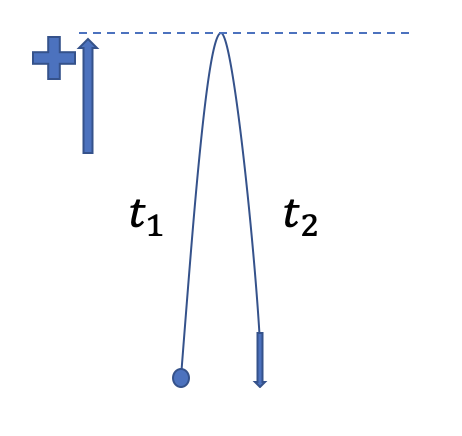
\includegraphics[width=4cm]{week4}
\end{figure}
In order to make content complete, first, let's consider the procedure without any friction.
\[mv^\prime=-mg
\]
\[v(t)=-gt+v_0\]
,where $v_0$ is a initial velocity.
\[v(T_{\textit{up}})=v_0-gT_{\textit{up}}
\]
\[T_{\textit{up}}=\frac{v_0}{g},~T_{\textit{down}}=\frac{v_0}{g}
\]
Now let's consider the case where air friction exists. By recent discovery, relationship between air friction and the speed of the objection is; $F=kv^{p}$ where $p$ ($
1\leq p\leq2$) is a constant related to the speed, i.e. when the speed is high, $p$ is aproximately 2; otherwise, $p$ is more close to 1 and $k$ is a constant related to the shape of the object.
\[F=-kv|v|
\](This hold nomatter $p$ is equal to 1 or 2 where $v$ is a vector.)
To make our life easier, take $p=1$,
\[mv^\prime=-mg-kv
\]
\[v^\prime=-g-\frac{k}{m}v
\]
Let $\rho=\frac{k}{m}$
\[v^\prime+\rho v=-g
\]
\[e^{\rho t}(v^\prime+\rho v)=-ge^{\rho t}\]
Take integral on both side of the equation,
\[e^{\rho t}v(t)-v(0)=-\int_0^tge^{\rho s}\diff s=-\frac{g}{\rho}(e^{\rho t}-1)
\]
\[e^{\rho t}v(t)=v_0+\frac{g}{\rho}-\frac{g}{\rho}e^{\rho t}
\]
\[v(t)=e^{-\rho t}(v_0+\frac{g}{\rho})-\frac{g}{\rho}
\]
\[v(T_{\textit{up}})=0=e^{-\rho T_{\textit{up}}}(v_0+\frac{g}{\rho})-\frac{g}{\rho}
\]
\[v_0+\frac{g}{\rho}=\frac{g}{\rho}e^{\rho T_{\textit{up}}}
\]
\[\boxed{e^{\rho T_{\textit{up}}}=\frac{v_0+\frac{g}{\rho}}{\frac{g}{\rho}}}
\]
Max height $H=\int_0^{T_{\textit{up}}}v(t)\diff t$
\[T_{\textit{down}}=T_{\textit{total}}-T_{\textit{up}}
\]
$T_{\textit{total}}$ is given by $h(T_{\textit{total}})=0$, where $h(t)=\int_0^tv(s)\diff s$
\[h(t)=\int_0^t[e^{\rho t}(v_0+\frac{g}{\rho})-\frac{g}{\rho}]\diff s=-\frac{1}{\rho}(e^{-\rho t}-1)(v_0+\frac{g}{\rho})-\frac{g}{\rho}t
\]
$h(total)=h(0)$ is given by $\frac{1}{\rho}(e^{-\rho T_{\textit{total}}}-1)(v_0+\frac{g}{\rho})=\frac{g}{\rho}T_{\textit{total}}$\\
Question: Can you see $T_{\textit{up}}<T_{\textit{down}}$?\\
Answer: Interesting.\\
$k=0$(no air)\\
$T_{\textit{up}}=\frac{v_0}{g}$
\[\begin{aligned}
H&=\int_0^{T_{\textit{up}}}(-gt+v_0)\diff t\\
&=(-\frac{g}{2}t^2+v_0t)|_0^{\frac{v_0}{g}}\\
&=\frac{v_0^2}{g}-\frac{g}{2}(\frac{v_0}{g})^2
=\frac{v_0^2}{2g}
\end{aligned}
\]
\[T_{\textit{total}}=2\frac{v_0}{g}
\]
$k>0$ $\quad T_{\textit{up}}=\frac{1}{\rho}ln(1+\frac{g}{\rho}v_0) \quad H=h_0+\frac{v_0}{\rho}-\frac{g}{\rho}T_{\textit{up}}$ \\
Question: please examine when $\rho\rightarrow 0$ everything goes to the right quantity.
\begin{example}
A bolt shot straight upward with initial velocity 49m/sec from a cross bow at ground level. With air resistance take into account. Assuming the constant $\rho=0.04$ (and $\rho=0.2$ for comparison). Compute $T_{\textit{up}}$ and $T_{\textit{down}}$.\\
$P=0.04$ $v_0=49$, $g=9.8m/sec^2$\\
\[T_{\textit{up}}=\frac{1}{0.04}ln(1+0.04\cdot5)=\frac{1}{0.04}ln(1.2)\approx4.56sec
\]
\[T_{\textit{total}}\approx9.41sec
\]
\[T_{\textit{down}}=9.41-4.56=4.85sec
\]
$p=0.2$
\[T_{\textit{up}}=3.47
\]
\[T_{\textit{total}}=8sec
\]
\[T_{\textit{down}}=4.53sec
\]
Indeed, upper time is shorter than downward time.

\end{example}


